\begin{frame}
\frametitle{A generative classification approach}
\begin{center}
\includegraphics[height=.8\textheight]{fld}
\end{center}
\end{frame}

\begin{frame}
\frametitle{Discriminative classification approaches}
\begin{center}
\includegraphics[height=.8\textheight]{linear_discrimination}
\end{center}
\end{frame}

\begin{frame}
\frametitle{Bayesian classification}
\begin{center}
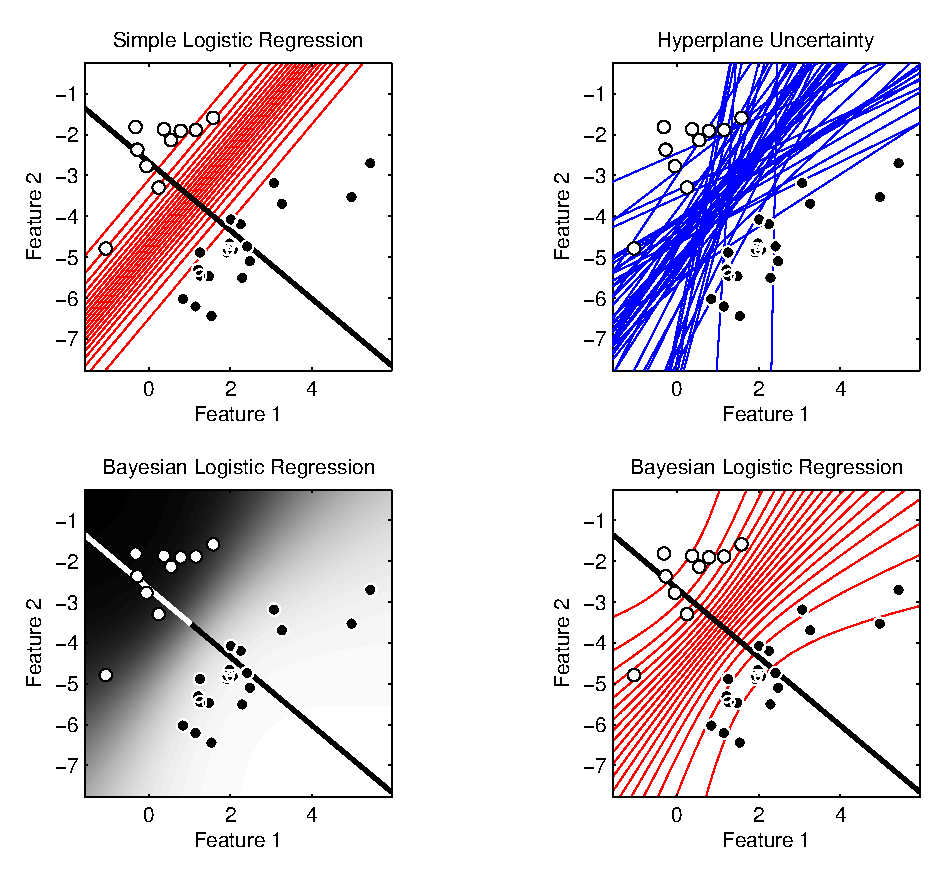
\includegraphics[height=.8\textheight]{logistic_regr}
\end{center}
\end{frame}

\begin{frame}
\frametitle{Why Bayesian?}
\begin{itemize}
\item To deal with different priors.
\begin{itemize}
\item Consider a method with 90\% sensitivity and specificity.
\item Consider using this to screen for a disease afflicting 1\% of the population.
\item On average, out of 100 people there would be 10 wrongly assigned to the disease group.
\item A positive diagnosis suggests only about a 10\% chance of having the disease.
{\small
\begin{eqnarray*}
P(\text{Disease} | \text{Pred+}) & = \frac{P(\text{Pred+} | \text{Disease}) P(\text{Disease})}{P(\text{Pred+} | \text{Disease}) P(\text{Disease}) + P(\text{Pred+} | \text{Healthy}) P(\text{Healthy})}\cr
 & = \frac{\text{Sensitivity} \times P(\text{Disease})}{\text{Sensitivity} \times P(\text{Disease}) + (1-Specificity) \times P(\text{Healthy})}
\end{eqnarray*}
\par
}
\end{itemize}
\item Better decision-making by accounting for utility functions.
\end{itemize}
\end{frame}

